\section{Introduction}\label{sec:intro}

% 核函数不特化 -> 性能变差 -> 现有核函数特化: 依赖 JIT 生成特化的核函数源码，

\begin{wrapfigure}{l}{0.48\textwidth}
    \centering
    \resizebox{\linewidth}{!}{
    \begin{tikzpicture}[node distance=1.2cm and 1.2cm]
        % Main Nodes
        \node[layeredbox] (dlsys) {DL Systems\nodepart{second}PyTorch, TF...};
        \node[layeredbox, right=1.5cm of dlsys] (ffi) {FFI\nodepart{second}pybind11...};

        % --- Upper Path: Specialized Library ---
        \node[simplebox, right=1.0cm of ffi, yshift=0.8cm] (cublashost) {Host};
        \node[simplebox, right=0.8cm of cublashost, yshift=0.3cm, minimum width=1.2cm] (k1) {Kernel 1};
        \node[simplebox, below=0.05cm of k1, minimum width=1.2cm] (k2) {Kernel 2};
        \node[simplebox, below=0.05cm of k2, minimum width=1.2cm] (kn) {...};
        
        % --- Lower Path: Generic Library ---
        \node[simplebox, right=1.0cm of ffi, yshift=-0.8cm] (cannhost) {Host};
        \node[simplebox, right=0.9cm of cannhost] (generic) {Generic\\[-4pt ]Kernels};

        % Grouping and Boxes
        \begin{scope}[on background layer]
            % Manual Specialized Library Enclosing Box (Upper)
            \node[enclosing_box, fit=(cublashost)(k1)(k2)(kn), minimum width=3.4cm] (cublas_path_box) {};
            \node[box_header, anchor=center, yshift=0.18cm, minimum width=3.4cm] (h1) at (cublas_path_box.north) {Specialized Library};
            % 独立数字 Node
            \node[number_icon, left=-0.6cm of h1.west] {\ding{182}};

            % Generic Library Enclosing Box (Lower)
            \node[enclosing_box, fit=(cannhost)(generic), minimum width=3.4cm] (cann_path_box) {};
            \node[box_header, anchor=center, yshift=0.18cm, minimum width=3.4cm] (h2) at (cann_path_box.north) {Generic Library};
            % 独立数字 Node
            \node[number_icon, left=-0.6cm of h2.west] {\ding{183}};
        \end{scope}

        % Connections
        \draw[stdarrow] (dlsys.east) -- 
            node[above, font=\sffamily\small, align=center, yshift=-0.5cm] {Runtime\\[0.1cm]Input} 
            (ffi.west);
        
        % Arrows for Specialized Library (Upper)
        \draw[stdarrow] (ffi.east) -- ++(0.3,0) |- (cublashost.west);
        \draw[stdarrow] (cublashost.east) -- ++(0.2,0) |- (k1.west);
        \draw[stdarrow] (cublashost.east) -- ++(0.2,0) |- (k2.west);
        \draw[stdarrow] (cublashost.east) -- ++(0.2,0) |- (kn.west);

        % Arrows for Generic Library (Lower)
        \draw[stdarrow] (ffi.east) -- ++(0.3,0) |- (cannhost.west);
        \draw[stdarrow] (cannhost) -- (generic);

        % Bubbles
        \node[bubble={($(cublas_path_box.north west)+(0,-0.15)$)}, left=0.3cm of cublas_path_box.north west, yshift=-0.1cm] (explosion) {
            Combinatorial Explosion~\raisebox{-0.3\height}{
\includegraphics[height=0.35cm]{figures/icons/boom.png}}
        };
        
        \node[bubble={($(cann_path_box.south west)+(0,0.3)$)}, above left=0.03cm and 0.3cm of cann_path_box.south west] (perf_loss) {
            Performance Loss~\raisebox{-0.3\height}{
\includegraphics[height=0.35cm]{figures/icons/down-arrow.png}}
        };
    \end{tikzpicture}
    }
    \caption{Comparison of different operator libraries. \ding{182} represents libraries involving manually specialized kernels and \ding{183} represents libraries that invoke general kernels without specialization.}
    \Description{Diagram comparing specialized library with combinatorial explosion and generic library with performance loss.}
    \label{fig:comparison-libraries}
\end{wrapfigure}

% 以 Pytorch, Tensorflow, vLLM, SGLang, ... 为代表的 DL系统为 DL 应用提供了高效的算子实现,促进了 DL 模型的落地部署.
% 支持 diverse model architectures, hyperparameter settings, and dynamic shapes 的通用算子库由于性能好、适配性强，在工业部署场景被广泛采用。
% 主流的通用算子库是基于类C的异构编程语言开发的通用程序，其中的算子需要在 Host 侧根据输入形状计算最优调度，传递到 Device 作为核函数的一部分输入。
% 然而，运行时处理这些与调度相关的输入(称作调度参数)会导致核函数性能显著下降。
% 这是因为编译期无法对核函数的调度参数(编译期变量)做积极的编译优化，例如常量折叠、循环展开、死代码删除等。
% 且随着底层高效算法和硬件架构的发展，融合算子的计算粒度越来越大，硬件内的可编程部件越来越多，调度参数越来越多，凸显了这种性能的下降。

% 尽管一些工作引入了特化核函数，但这些方法无法推广到各种算子库。
% 图 1 给出了 common scenarios in which a DL 系统调用 AI Compiler 生成的特化算子或者调用 Vendor library 中的算子。
% 以 Triton 为代表的 AI Compiler 通过即时编译（JIT）利用运行时信息进行特化，但其依赖特定的高层语言抽象，难以直接应用于广泛存在的、用类 C 异构语言编写的底层算子库。
% 以 cuBLAS 为代表的算子库方案依赖 C++ 模板与人工编写的分派逻辑，这不仅要求开发者预先定义复杂的特化规则，而且在面对大量可调参数时，会陷入组合爆炸的困境，导致难以实现覆盖所有参数的充分特化。

% 静态地实现算子库核函数的自动特化，需要追踪数据在全栈中的流向：从顶层的深度学习模型代码出发，穿过框架复杂的 Python/C++ 绑定接口，经由算子库内部的调度计算，最终映射到底层核函数的常量参数上。
% 这种跨语言、全链路的值流分析对于支持诸如编译时常量折叠和高性能代码生成等优化任务至关重要。
% 然而，现有的静态分析方法均无法有效捕获这些穿越深度学习系统各层级的关键值流。
% 这一挑战主要源于深度学习框架极高的集成复杂度，其涉及的算子调度往往受到动态张量形状、硬件后端属性以及运行时推理配置的影响。
% 解析这些流向必须建模 Python 对象经由绑定接口到 C++ 内部结构的值流映射，并准确模拟 C++ 侧复杂的算子调度的行为。

% 为了构建自动化的算子特化，我们依赖于跨语言常量传播，这是一种旨在捕捉跨语言边界值流的基础静态分析技术。
% 据此，我们提出了 \mysys，这是首个设计用于统一分析深度学习软件栈中的常量值流传播，并实现算子库程序自动特化的系统。
% \mysys 由三个主要组件构成：
% (1) Context Generation 模块，它通过分析绑定代码的 AST 并应用基于规则的建模来构建初始的 operator context，从而弥合语义鸿沟；
% (2) Information Propagation 引擎，它利用提前返回（early return）识别来剪枝无效路径，并执行上下文敏感的过程间分析以在复杂的 Host 端程序中传播常量——具体而言，它集成了指向集（points-to set）传播以解决指针别名问题，并对循环采用混合模拟策略，同时利用现有的别名分析来约束未知指针的弱更新以确保内存精度；
% (3) Kernel Specializer，它利用推断出的不变量（invariants）对核函数的 LLVM IR 进行特化，生成高度优化的二进制代码以替换通用核函数。\mysys 的每个组件都通过引入针对 DL 系统混合语言环境的特定机制，对传统静态分析进行了扩展。
% 这使得 \mysys 能够解决从运行时框架到静态编译器传播常量的复杂性，支持自动核函数调优和库优化等任务，从而显著提升深度学习模型的运行时性能。综上所述，本文做出了以下贡献。
% 总结来说，贡献如下：
% item 1: 我们提出



% 尽管现有的工作试图通过代码生成或模板特化来缓解这一性能损耗，但它们在通用性和自动化程度上仍存在局限。
% 以 Triton 为代表的 DSL 方案通过即时编译（JIT）利用运行时信息进行特化，但其依赖特定的高层语言抽象，难以直接应用于广泛存在的、用类 C 异构语言编写的底层算子库，且往往难以达到手工优化代码的极致性能。
% 另一方面，以 FlashInfer 为代表的算子库方案依赖 C++ 模板与人工编写的分派逻辑，这不仅要求开发者预先定义复杂的特化规则，而且在面对大量可调参数时，会陷入组合爆炸的困境，导致难以实现覆盖所有参数的充分特化。
% 因此，当前针对算子特化领域仍缺乏一种能够面向通用算子库、无需人工干预即可实现自动核函数常量特化的机制。


% tracing the flow of data from app code,
% through various database access APIs in frameworks, via SQL manipulations, to the database, and
% then back to the app code.
% 主要挑战在于DL系统通过跨语言调用算子程序


Deep Learning (DL) models are typically deployed using DL systems~\cite{ansel2024dynamo,abadi2016tensorflow,kwon2023vllm,zheng2024sglang} that rely on libraries of C++ generic operators~\cite{nvidia2021cublas,nvidia2017cutlass,ye2025flashinfer,HuaweiCANN}. 
In this paradigm, a model is represented as a Directed Acyclic Graph (DAG), where nodes represent operators and edges represent tensor data dependencies. 
The system executes these nodes in topological order by invoking the corresponding C++ operator programs.
These operators are designed to be \texttt{generic} to adapt to diverse model architectures, hyperparameter settings, and dynamic shapes. 
For example, query lengths and KV caches vary within batches and over time for LLMs~\cite{vaswani2017attention,yang2024qwen2technicalreport,touvron2023llama2openfoundation}, while batch sizes vary in computer vision models~\cite{he2016resnet,redmon2018yolov3}.
To handle such dynamics, the host-side (CPU) program calculates execution parameters, such as tiling sizes and block dimensions, based on runtime inputs. 
These parameters are then passed to the device-side kernel, referred to as a \texttt{generic kernel}. 
For instance, \autoref{lst:add_kernel_with_formal_param} shows a simple kernel of operator \kw{add}, where \kw{s} represents a dynamic dimension size and \kw{t} denotes the tiling size, both defined as formal parameters passed from the host.

\begin{figure}[htbp]
    \centering
    \begin{minipage}{0.48\textwidth}
    \begin{lstlisting}[basicstyle=\ttfamily\footnotesize, frame=single]
void kernel(float* A, float* B, float* C, int s, int t) {
  for (int i = 0; i < s; i += t)
    for (int j = 0; j < t; ++j)
      int idx = i + j;
      if(idx < s) C[idx] = A[idx] + B[idx];
}
    \end{lstlisting}
    \end{minipage}
\hfill
    \begin{minipage}{0.48\textwidth}
    \begin{lstlisting}[basicstyle=\ttfamily\footnotesize, frame=single, firstnumber=7]
status add(Tensor& A, Tensor& B, Tensor& C) {
  int s = A.size(0), t = 0;
  if (tiling(s, t) != SUCCESS) 
    return ERROR;
  kernel(A.ptr, B.ptr, C.ptr, s, t);
}
    \end{lstlisting}
    \end{minipage}
    \caption{Example of the add operator. Parameters \kw{s} and \kw{t} represent the size of the input tensors and the tiling factor, respectively. 
    The \kw{tiling} function computes the tiling factor based on the input size. 
    The \kw{add} function serves as the operator interface, extracting input sizes and invoking the kernel with the appropriate parameters. 
    For simplicity, the definition of the \kw{tiling} function is shown in \autoref{lst:early_return_code}. 
    \texttt{Tensor} is a data structure representing a multi-dimensional array adopted in deep learning frameworks, with a method \texttt{size} that retrieves the size of a specific dimension.}
    \Description{}
    \label{lst:add_kernel_with_formal_param}
\end{figure}

However, relying on generic kernels introduces significant challenges in the era of specialized AI accelerators.
While Just-In-Time (JIT) compilation approaches (e.g., Triton~\cite{tillet2019triton}, TVM~\cite{chen2018tvm}) have emerged to generate kernels automatically, production environments often prioritize vendor-provided operator libraries (e.g., CuBLAS~\cite{nvidia2021cublas}, CANN~\cite{HuaweiCANN}) because they contain hand-tuned micro-architecture optimizations that are difficult for automated compilers to replicate.
As algorithms grow in complexity~\cite{dao2024flashattention2,dong2025flexattention,ye2025flashinfer,flashmla2025,aimuyo2025FlashMoE}, preserving the "generic" nature of these libraries requires passing an increasing number of parameters to control the device-side execution.
This creates substantial overhead on accelerators with decoupled scalar-vector architectures, such as the Ascend NPU~\cite{liao2019davinci} and other many-core processors.
In these architectures, the scalar unit is responsible for handling control flow and parameter dispatch, while the vector/cube units handle heavy computation.
Mapping complex scheduling decisions to kernel parameters leads to parameter explosion, which can saturate the scalar unit and cause pipeline stalls.
\autoref{lst:scalar_ratio_icache_miss} uses the Qwen2-1.5B~\cite{yang2024qwen2technicalreport} model on the Ascend 910B1 NPU to illustrate this issue:
(1) \textbf{Scalar Unit Saturation:} The scalar unit is active for 85\% of cycles handling instruction dispatch and control logic, leaving insufficient headroom for efficient pipelining with compute units.
(2) \textbf{Instruction Cache Pressure:} The complex control flow required to support generic adaptation increases instruction cache misses.
Consequently, generic kernels perform consistently worse than fully specialized kernels, where variable parameters are instantiated as compile-time constants, with performance gaps exceeding 10\% on complex operators.

\begin{figure}[htbp]
    \centering
    \begin{minipage}{0.45\textwidth}
        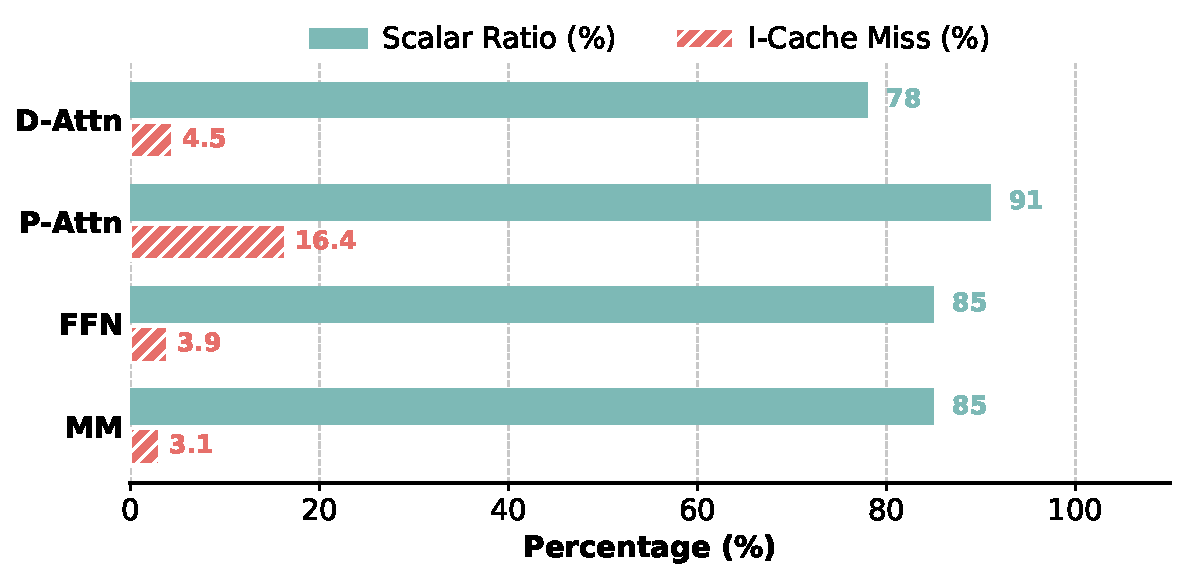
\includegraphics[width=0.95\linewidth]{figures/motivation/metrics_analysis.pdf}
        \caption{Four representative operators used in Qwen2 show high scalar unit utilization and instruction cache miss rates, indicating significant overhead from generic control flows.}
        \label{lst:scalar_ratio_icache_miss}
    \end{minipage}
    \hfill
    \begin{minipage}{0.45\textwidth}
        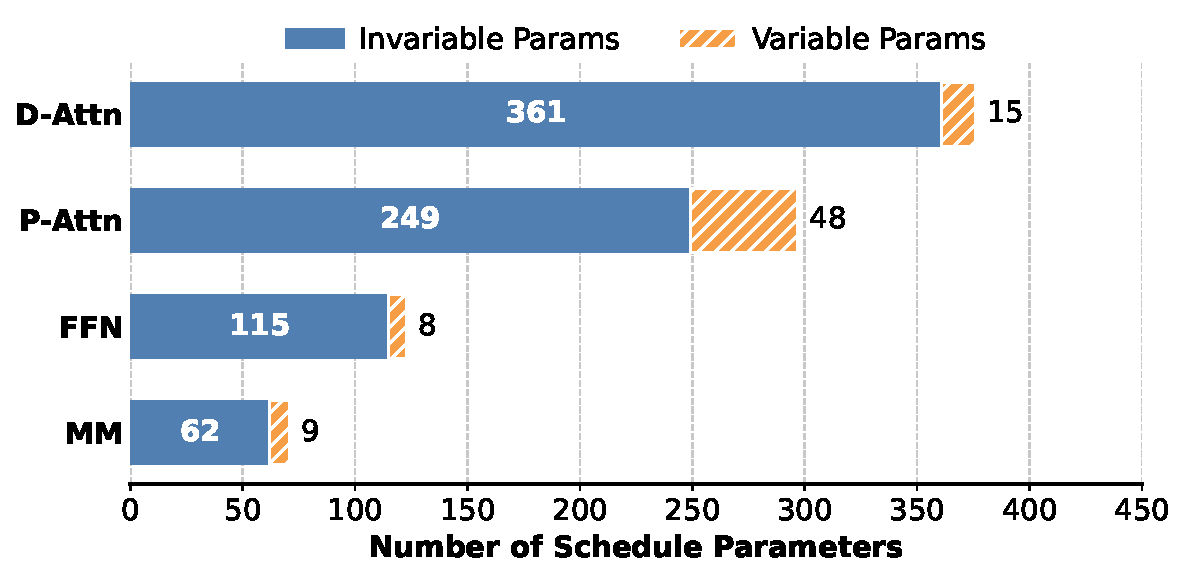
\includegraphics[width=0.95\linewidth]{figures/motivation/parameter_breakdown.pdf}
        \caption{Although the number of kernel parameters is large, the majority remain invariable at runtime for a specific model deployment.}
        \label{lst:invariable_params}
    \end{minipage}
\end{figure}

% \definecolor{bordergray}{RGB}{180, 180, 180}
% \definecolor{headerblue}{RGB}{220, 230, 240}
% \definecolor{paleblue}{RGB}{240, 248, 255}
% \definecolor{codekey}{RGB}{0, 0, 255}
% \definecolor{codestr}{RGB}{163, 21, 21}
% \definecolor{flowred}{RGB}{220, 50, 47}
% \definecolor{flowblue}{RGB}{38, 139, 210}
% \definecolor{llvmgreen}{RGB}{0, 100, 0}

% \tikzset{
%     % 基础面板
%     panel_base/.style={
%         draw=bordergray,
%         thick,
%         fill=white,
%         inner sep=3pt,
%         align=left,
%         anchor=north west,
%         outer sep=0pt
%     },
%     panel_slim/.style={ panel_base, text width=2.8cm, inner sep=2pt, outer sep=0pt},
%     panel_narrow/.style={ panel_base, text width=4.0cm, inner sep=2pt, outer sep=0pt},
%     panel_wide/.style={ panel_base, text width=5.2cm, inner sep=2pt, outer sep=0pt},
%     % 虚线背景面板 (去掉了 fill=paleblue，实现无底纹)
%     panel_dashed/.style={
%         draw=bordergray,
%         thick,
%         dashed,
%         % fill=paleblue, % 已注释掉背景色
%         inner sep=2pt,
%         align=left,
%         anchor=north west,
%         outer sep=0pt
%     },
%     % 标题栏样式
%     header/.style={
%         fill=headerblue,
%         draw=bordergray,
%         thick,
%         align=center,
%         font=\bfseries\scriptsize,
%         yshift=-0.5pt,
%         outer sep=0pt,
%         inner sep=2pt,
%         anchor=south west
%     },
%     % 连线样式
%     flowline/.style={->, >=stealth, thick, rounded corners=2pt},
%     typearrow/.style={->, >=stealth, dashed, thick, color=gray},
%     % 变量高亮框
%     boxstyle/.style={draw, thick, rounded corners=1pt}
% }

% \newcommand{\tightnode}[3][]{%
%     \tikzmarknode[%
%         inner xsep=1.5pt,
%         inner ysep=0.5pt,
%         text height=6.0pt,
%         text depth=1.5pt,
%         #1  % <-- 允许插入额外的样式覆盖默认设置
%     ]{#2}{%
%         \smash{#3}
%     }%
% }

% \lstset{
%     language=C++,
%     basicstyle=\ttfamily\fontsize{5pt}{6pt}\selectfont,
%     breaklines=true,
%     escapechar=@, 
%     numbers=left,
%     numberstyle=\tiny\color{gray!50},
%     numbersep=2pt,
%     keywordstyle=\color{codekey}\bfseries,
%     commentstyle=\color{gray},
%     stringstyle=\color{codestr},
%     showstringspaces=false,
%     frame=none,
%     xleftmargin=0.8em,
%     lineskip=-0.5pt,      
%     aboveskip=2pt,        
%     belowskip=0pt
% }

% \begin{figure}[htbp]
%     \centering
%     \begin{tikzpicture}[remember picture]
        
%         % ==========================
%         % 1. PyTorch Frontend (Python)
%         % ==========================
%         \node[panel_slim, text width=2.8cm] (p1) {
%         % --- Part A: ATen IR (Compiler View) ---
%         \textbf{\scriptsize\sffamily\color{black} [Compile Time / ATen IR]} \\
%         \begin{lstlisting}[language=llvm]
% %B: SymInt
% %S: SymInt
% %lens: Array(SymInt)
% %q: Tensor[%B,@\tightnode{initial_const}{40}@,%S,64]
% %out = aten::fa(%q, 
%   %k, %v, %lens, ...)
%         \end{lstlisting}
        
%         \vspace{2pt}
%         \color{gray}\hrule height 0.5pt \normalcolor
%         \vspace{2pt}
        
%         % --- Part B: Python API (User View) ---
%         \textbf{\scriptsize\sffamily\color{black} [Runtime / Op Invocation]} \\
%         \begin{lstlisting}[language=Python]
% while greedy_search:
%   ...
%   # lens grows
%   torch.fa(q_cur, k_cache, v_cache, @\tightnode{py_seq}{lens}@, ...)
%         \end{lstlisting}
%     };
%         \node[header, text width=2.8cm] at (p1.north west) {1. PyTorch (Python)};
        
%         % ==========================
%         % 2. PyBind Schema (C++)
%         % ==========================
%         \node[panel_slim, text width=2.8cm, right=0.3cm of p1.north east, anchor=north west] (p2) {
%      \begin{lstlisting}[language=C++]
% struct Tensor { 
%   void* data_;
%   int* sizes; 
%   int ndim; 
% };
% m.def("fa", [](
%   Tensor @\tightnode{pb_q}{q}@, ..., 
%   int[] @\tightnode{pb_seq}{s}@, ...) {
%   return host_fa(q, k, v, s, ...);
% });
%     \end{lstlisting}
%         };
%         \node[header, text width=2.8cm] at (p2.north west) {2. PyBind (C++)};

%         % ==========================
%         % 3. Host Runtime (C++)
%         % ==========================
%         \node[panel_narrow, text width=4.0cm, right=0.3cm of p2.north east, anchor=north west] (p3) {
%         \begin{lstlisting}
% Tensor host_fa(Tensor q, ...){
%  int h = @\tightnode{host_h}{q}@.size(1); // 40
%  int stages = (@\tightnode{host_stages}{h}@>32)? @\tightnode{llvm_s_val}{2}@ : 1;
%  EXEC(kernel, ..., stages, @\tightnode{host_lens}{sum(s)}@);
% }
%         \end{lstlisting}
%         };
%         \node[header, text width=4.0cm] at (p3.north west) {3. Host (C++)};

%         % ==========================
%         % 4. Device Kernel
%         % ==========================
%         \node[panel_wide, text width=4.0cm, right=0.3cm of p3.north east, anchor=north west] (p4) {
%             \begin{lstlisting}
% void kernel(..., int stages, int len_sum) {
%   if (tid >= @\tightnode{kern_lens}{len\_sum}@) return;
%   for(int i=0; i < @\tightnode{kern_stages}{stages}@; i++)
%     ...
% }
%             \end{lstlisting}
%         };
%         \node[header, text width=4.0cm] at (p4.north west) {4a. Generic Kernel (C++)};

%         \node[panel_wide, text width=3.6cm, below=0.8cm of p4.south east, anchor=north east] (p_spec) {
%         \begin{lstlisting}
% void kernel(..., int len_sum) {
%   if (tid >= @\tightnode{kern_lens_use}{len\_sum}@) return; 
%   @\tightnode[inner sep=3pt]{kern_stage_spec}{%
%     \begin{tabular}{@{}l@{}}
%       ... // Stage 1\\
%       ... // Stage 2
%     \end{tabular}%
%   }@
% }
%         \end{lstlisting}
%         };
%         \node[header, text width=3.6cm] (p_spec_header) at (p_spec.north west) {4b. Specialized Kernel (C++)};

%         % ==========================
%         % 3.5 LLVM IR (JIT Analysis)
%         % ==========================
%         \node[panel_dashed, text width=4.4cm, below=0.8cm of p3.south west, anchor=north west] (p_llvm) {
%         \begin{lstlisting}[language=llvm]
% ...
% sizes = getelementptr %q ...
% h_ptr = getelementptr %sizes, i32 4
% h_val = load i32, %h_ptr  ; Load 40
% cmp = icmp sgt i32 %h_val, 32
% stages = select i1 %cmp, i32 2, i32 1
%         \end{lstlisting}
%         };
%         \node[header, text width=4.4cm] (p_llvm_header) at (p_llvm.north west) {3. Propagation on LLVM IR of Host};

% %         % ==========================
% %         % Type Mapping Layer - MODIFIED
% %         % ==========================
% %         \node[panel_dashed, text width=6cm, anchor=north west] (p_typemap) at (p1.south west |- p_llvm.north west) {
% %             \vspace{2pt} % Leave space for header
% %             \begin{minipage}{0.35\textwidth}
% %             \begin{lstlisting}[basicstyle=\ttfamily\tiny, numbers=none]
% % // C++ Layout            
% % struct Tensor {
% %  void* data_;
% %  int* sizes;
% %  int ndim;
% % };
% %             \end{lstlisting}
% %             \end{minipage}%
% %             \hfill
% %             \begin{minipage}{0.63\textwidth}
% %             \begin{lstlisting}[basicstyle=\ttfamily\tiny, numbers=none]
% % // PyBind Registration
% % py::class_<Tensor>(m, "Tensor")
% %   .def("size", [](Tensor& t, int id){ 
% %     return t.sizes[id]; 
% %  });
% %             \end{lstlisting}
% %             \end{minipage}
% %         };
% %         % Added Header for Type Mapping Layer
% %         \node[header, text width=6cm] (p_typemap_header) at (p_typemap.north west) {Type Mapping Layer (Python $\leftrightarrow$ C++)};

%     \end{tikzpicture}

%     % --- 绘制连线 (Overlay) ---
%     \begin{tikzpicture}[remember picture, overlay]
        
%         % --- RED FLOW: Metadata/Constant Flow ---
%         % 1. Python (40) SE -> PyBind (q) NW
%         \draw[flowred, boxstyle] (initial_const.north west) rectangle (initial_const.south east);
%         \draw[flowred, boxstyle] (pb_q.north west) rectangle (pb_q.south east);
%         \draw[flowline, flowred] (initial_const.north east) -- ++(1,0) |- (pb_q.north west);
        
%         % 2. PyBind (q) SE -> Host (q) NW
%         \draw[flowred, boxstyle] (host_h.north west) rectangle (host_h.south east);
%         \draw[flowline, flowred] (pb_q.north east) -- ++(1,0) |- (host_h.north west);
        
%         % 3. Host (q) SW -> Host (S) NE
%         \draw[flowred, boxstyle] (host_stages.north west) rectangle (host_stages.south east);
%         \draw[flowline, flowred] (host_h.south west) -- (host_stages.north west);

%         % 4. Host (S) -> LLVM / Device (IR Generation)
%         % \draw[flowline, flowred, dashed, opacity=0.5] (host_stages.south) -- (p_llvm_header.north);

%         % 5. LLVM -> Device Specialization
%         \draw[flowred, boxstyle] (llvm_s_val.north west) rectangle (llvm_s_val.south east);
%         \draw[flowred, boxstyle] (kern_stages.north west) rectangle (kern_stages.south east);
%         \draw[flowline, flowred] (llvm_s_val.south east) -- ++(1,0) |- (kern_stages.south west);

%         % --- BLUE FLOW: Variable Flow (Lens) ---
%         % 1. PyTorch -> PyBind
%         \draw[flowblue, boxstyle] (py_seq.north west) rectangle (py_seq.south east);
%         \draw[flowblue, boxstyle] (pb_seq.north west) rectangle (pb_seq.south east);
%         \draw[flowline, flowblue] (py_seq.north east) -- ++(1.5,0) |- (pb_seq.south west);

%         % 2. PyBind -> Host
%         \draw[flowblue, boxstyle] (host_lens.north west) rectangle (host_lens.south east);
%         \draw[flowline, flowblue] (pb_seq.south east) -- ++(1.8,0) |- (host_lens.north west);

%         % 3. Host -> Kernel (Argument)
%         \draw[flowblue, boxstyle] (kern_lens.north west) rectangle (kern_lens.south east);
%         \draw[flowline, flowblue] (host_lens.north east) -- ++(2,0) |- (kern_lens.south west);
        
%         % 4. Kernel Argument -> Usage
%         \draw[flowblue, boxstyle] (kern_lens_use.north west) rectangle (kern_lens_use.south east);
%         \draw[flowred, boxstyle] (kern_stage_spec.north west) rectangle (kern_stage_spec.south east);
%         % \draw[->, flowblue, dotted, thick] (kern_lens.south) -- ++(0,-0.3) -| (kern_lens_use.north);

%         % --- GREY ARROW: Type Mapping Relationship ---
%         % \draw[typearrow] (p1.south) -- node[left, font=\tiny, text=gray] {PyObject} (p_typemap_header.north -| p1.south);
%         % \draw[typearrow] (p_typemap_header.north -| p2.south) -- node[right, font=\tiny, text=gray] {C++ Struct} (p2.south);
%         \draw[typearrow] (p3.south -| p_llvm_header.south) -- node[right, font=\tiny, text=gray] {IR Generation} (p_llvm_header.north);
%         \draw[flowline, flowred] (p4.south -| p_spec_header.south) -- node[right, font=\tiny, text=flowred] {Specialization} (p_spec_header.north);

%     \end{tikzpicture}
%     \caption{Flash Attention Optimization Flow: Constant Propagation \& Field Reconstruction.}
% \end{figure}



In practice, however, the vast majority of kernel parameters remain invariant during a specific model deployment.
\autoref{lst:invariable_params} demonstrates that when deploying Qwen2-1.5B on Ascend 910B1, over 90\% of parameters remain constant given 100 randomly generated inputs with different shapes.
This reveals a significant optimization opportunity: if we can identify these invariants and substitute them with immediate values, we can generate specialized kernels that retain the hand-written optimizations of vendor libraries while eliminating the overhead of generic parameter handling.

Based on these observations, we propose \mysys, a compilation framework that specializes library kernels using static analysis during graph compilation.
Unlike JIT compilers that generate code from scratch, \mysys focuses on specializing \texttt{existing} C++ DL operator libraries.
This allows it to inherit the micro-architectural optimizations of vendor libraries while gaining the performance benefits of specialization.
However, identifying parameter invariants by propagating information through C++ operator programs is non-trivial. 
Achieving this target faces two unique challenges arising from the cross-language architecture and the dynamic semantics of generic operators.

\textbf{Cross-Language Semantic Loss.} 
Effective specialization necessitates a precise calling context, specifically the physical memory layout and runtime values of C++ arguments. 
However, modern DL systems rely on a foreign function interface (FFI) layer to invoke C++ functions within a Python-based framework.
Static analysis cannot easily traverse this layer to simulate the construction logic of C++ objects.
Without a clear mapping between Python symbolic variables (e.g., dynamic shapes) and C++ memory offsets, the analyzer cannot distinguish constants from variables, blocking effective constant propagation.

\textbf{Patterns of Validation Checks.}
Generic operator programs extensively validate inputs to detect errors such as dimension mismatch.
Upon failure, the program triggers an \texttt{early return}, skipping the normal execution path.
These validation checks create multi-path propagation complexities.
Consequently, it becomes difficult for the analyzer to determine the deterministic constant values used in the \texttt{normal} execution path at the final kernel call site.

\mysys addresses these challenges to achieve precise kernel specialization through two core designs:
First, we introduce rule-based cross-language modeling. 
Instead of manually writing rules for every operator, \mysys defines mapping rules for core data structures (e.g., \texttt{Tensor}, \texttt{Context}) that bridge high-level Python attributes to C++ memory layouts. 
This reconstructs a field-sensitive calling context for static analysis that is applicable across all operators using these structures.
Second, we propose a semantic check for early return recognition. 
This mechanism traces error codes through the Control Flow Graph (CFG) to identify and prune edges associated with validation failures, ensuring the analysis focuses on the valid execution flow.

\begin{figure}
    \centering
    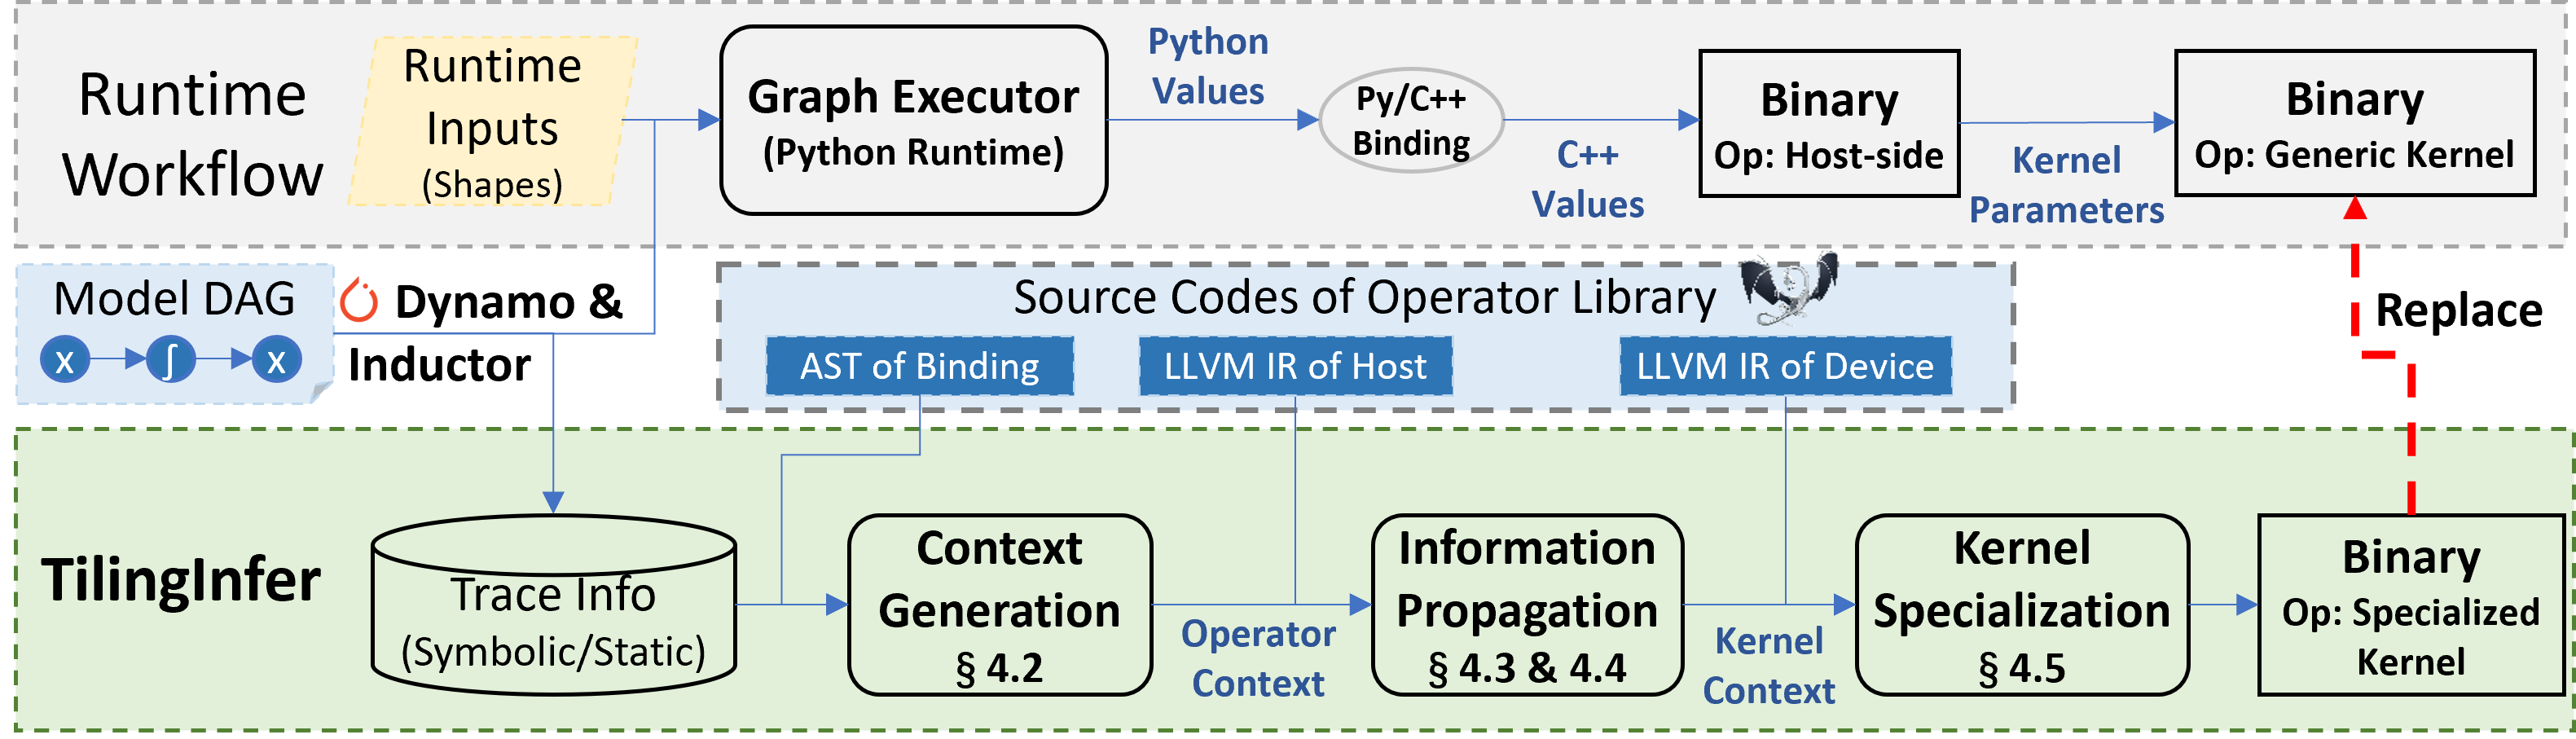
\includegraphics[width=\linewidth]{figures/intro/TilingInfer-overflow.png}
    \caption{Overview of \mysys design}
    \Description{}
    \label{fig:sys-design}
\end{figure}

\autoref{fig:sys-design} presents an overview of the \mysys workflow integrated into the deep learning compiler stack of PyTorch~\cite{ansel2024dynamo}. 
The process begins by leveraging trace information captured by the DL system. 
\mysys then proceeds through three phases:
(1) \textbf{Context Generation}: 
It bridges the semantic gap by analyzing the AST of bindings and applying rule-based modeling to construct an initial \texttt{operator context}.
(2) \textbf{Information Propagation}: 
This phase employs early return recognition to prune invalid paths and executes a context-sensitive inter-procedural analysis to propagate constants through complex host-side programs. 
Specifically, it integrates points-to set propagation to resolve pointer alias and adopts a hybrid simulation strategy for loops. 
To ensure memory precision, it leverages existing alias analysis to further constrain weak updates for unknown pointers.
(3) \textbf{Kernel Specialization}: Finally, using the inferred invariants, \mysys specializes the LLVM IR of kernel functions, generating a highly optimized binary to replace the generic kernel.

In summary, this paper makes the following contributions:
\begin{itemize}
    \item \textbf{Performance Analysis of Generic Kernels:} We identify that the overhead of dynamic shape operators on decoupled architectures (like Ascend NPUs) stems from scalar unit saturation and instruction cache misses. We further observe that the majority of these kernel parameters are invariant during runtime.
    \item \textbf{Automated Library Specialization:} We propose \mysys, a framework that specializes existing C++ libraries by solving FFI and validation challenges via rule-based cross-language modeling and early return recognition. 
    Underlying these techniques is a context-sensitive inter-procedural analysis on LLVM IR that integrates points-to set propagation and hybrid loop simulation to robustly propagate constants through complex C++ programs.
    \item \textbf{Evaluation and Impact:} We implement \mysys on the Ascend platform. Experiments show an average speedup of 1.06$\times$ (up to 1.17$\times$) on operators and 1.03$\times$ end-to-end speedup on LLM inference. Furthermore, we demonstrate the generalization of \mysys by applying it to GPU libraries, where it successfully debloats binary sizes by over 96\%, proving its utility across different hardware architectures.
\end{itemize}